\documentclass{article}

\usepackage[backend=biber]{biblatex}
\usepackage[hidelinks]{hyperref}
\usepackage{tikz}
\usepackage{mathtools,amssymb,amsthm,mathpartir,fitch}
\usepackage[llbracket,rrbracket]{stmaryrd}
\usepackage{listings}

\bibliography{sources.bib}

\newtheorem{theorem}{Theorem}
\newtheorem{lemma}[theorem]{Lemma}
\theoremstyle{definition}\newtheorem{definition}{Definition}

\newcommand{\lock}{\text{\tikz[baseline]{
      \fill[rounded corners=.1ex] (-.75ex,0) rectangle (.75ex,1ex);
      \draw[line width=.3ex] (-.4ex,.5ex) -- ++(0,.75ex) arc (180:0:.4ex) -- ++(0,-.75ex);
}}}

\DeclareMathOperator\Rpl{Rpl}
\DeclareMathOperator\unbox{unbox}

\begin{document}

\begin{titlepage}\centering

{\scshape\LARGE Master Thesis Half-Time Report\\}

\vspace{0.5cm}

{\huge\bfseries A Parametric Fitch-Style Modal Lambda Calculus\\}

\vspace{2cm}

{\Large Axel Forsman \texttt{<foraxel@student.chalmers.se>} \\}

\vspace{1.0cm}

{\large Supervisor: Nachiappan Valliappan \\}

\vspace{1.0cm}

{\large Examiner: Andreas Abel \\}

\vspace{1.5cm}

{\large Relevant completed courses:\par}

{\itshape \begin{itemize}
  \item DAT060, Logic in Computer Science; and
  \item DAT350, Types for Programs and Proofs.
  \end{itemize}}

\vfill
{\large April 17, 2023 \\}
\end{titlepage}

\section{Introduction}

The \emph{necessity modality}, denoted by $\Box$, where the focus will lie,
has been applied to model confidentiality in information-flow control,
compartmental purity in functional languages,
and more.
For a formula $\phi$, the formula $\Box \phi$ reads
``It is necessarily true that $\phi$'' -
$\Box$ changes the \emph{mode} of $\phi$.
So called Fitch-style modal deduction,
where modalities are eliminated by opening a subproof,
and introduced by shutting one,
has been adapted for lambda calculi.
Different modal logics may be encoded via different open and shut rules.
Prior work \cite{valliappan22} has given normalization proofs
for four Fitch-style formulations of lambda calculi with different modalities,
which required repeating the proofs for each individual calculus.
This prompts the need for a parametric Fitch-style modal lambda calculus
generalizing the variants,
in order to avoid repetition and ease further extensions.

This thesis is structured as follows:
\autoref{sec:background} contains an overview of the theory underlying the work;
and \autoref{sec:calculus} and \autoref{sec:normalization}
present the main result of this thesis,
the parametric calculus and a accompanying normalization algorithm.
In \autoref{sec:correctness} the correctness of normalization is proved;
and \autoref{sec:instantiations} gives two concrete instantiations
of the parametric calculus.
Finally \autoref{sec:conclusion} concludes by discussing
relations to prior work and possible future work.

\section{Background}\label{sec:background}

In this section we summarize the necessary background knowledge
for understanding the rest of the material.

\subsection{Modal natural deduction}

Modalities originate from modal logic.
Here we consider the family of modal logics
derived from intuitionistic propositional logic
extended with the unary connective $\Box$,
the inference rule \emph{necessitation},
if $A$ then $\Box A$,
and different axioms surrounding $\Box$ \cite{clouston18}.
The most basic modal calculi, IK, comes from the \emph{K axiom}
($\Box (A \supset B) \supset \Box A \supset \Box B$).
K together with \emph{axiom T} ($\Box A \supset A$) gives IT;
K and \emph{axiom 4} ($\Box A \supset \Box\Box A$) yield IK4;
and K, T and 4 give IS4.

Natural deduction is a proof system
wherein reasoning is carried out using ``natural'' inference rules.
\textcite{fitch52} introduced a notation for propositional natural deduction,
central to which is the idea of \emph{subordinate proof}.
For example, in order to prove ``$A$ implies $B$,'' $A \supset B$,
a subordinate proof may be opened containing the new assumption $A$,
where one sets out to prove $B$.
If successful, the subordinate proof can be shut
by introducing $A \supset B$ in the original proof
thereby discharging the assumption $A$.

This may be understood using Kripke's possible worlds interpretation \cite{kripke63, huth04}.
Opening a subproof means visiting a replica new world,
with an increase in knowledge owing to the new assumption,
and shutting means returning.

To extend natural deduction to modal logic,
Fitch added the notion of a \emph{strict} subordinate proof \cite{borghuis94},
see the example in \autoref{fig:ex-modal-nat-deduction},
indicated by a `$\Box$' to the left of the line delineating the subproof.
It is differentiated by not
introducing a new hypothesis for the antecedent of the implication.
Additionally,
strict subordinate proofs may access
prior derived formulas only of a certain shape
from proofs to which they are subordinate.
This is in contrast to ``ordinary'' subordinate proofs
wherein any previous formula from a outer proof may be reiterated.
This is how the mixing of formulas of different modes is prevented.
Their usage is given in the following two rules for the logic K:
\begin{equation*}
  \begin{array}{l@{\hskip 4em}l}
    \textsc{K-Import} & \textsc{K-Export} \\
    \begin{fitch*}
      \Box \varphi \\
      \vdotswithin{\Box \varphi} \\
      \fn \vdotswithin{\varphi} \\
      \fa \varphi
    \end{fitch*} &
    \begin{fitch*}
      \fn \vdotswithin{\varphi} \\
      \fa \varphi \\
      \Box \varphi
    \end{fitch*}
  \end{array}
\end{equation*}
With \textsc{K-Import} we may import boxed formulas,
but after we are done reasoning about them we must re-box the result
with \textsc{K-Export} to make use of it.

\begin{figure}
  \centering
    \begin{fitch}
      \fj \Box (A \supset B) \\
      \fa \fh \Box A \\
      \fa \fa \fn A \supset B & K-import, 1 \\
      \fa \fa \fa A & K-import, 2 \\
      \fa \fa \fa B & $\supset$-elim, 3, 4 \\
      \fa \fa \Box B & K-export, 3-5 \\
      \fa \Box A \supset \Box B & $\supset$-intro, 2-6 \\
      \Box (A \supset B) \supset (\Box A \supset \Box B) & $\supset$-intro, 1-7
    \end{fitch}
  \caption{Example of a modal natural deduction proof of the formula
    $\Box (A \supset B) \supset (\Box A \supset \Box B)$.
    Note how a strict subordinate proof must be opened
    in order to facilitate reasoning about that inside modalities.
    \label{fig:ex-modal-nat-deduction}}
\end{figure}

\subsection{Lambda calculus with modalities}

The Curry-Howard isomorphism \cite{howard80} connects logic and lambda calculus,
a bare-bones model of computation
consisting of only functions and function application.
The grammar of lambda calculus terms is evidently short:
\begin{align*}
  t, s \Coloneqq& \, x &&\text{variable access} \\
  \mid& \, \lambda x.\, t &&\text{lambda abstraction} \\
  \mid& \, t \; s &&\text{function application}
\end{align*}
The isomorphism states that there is a correspondence between
formulae and their proofs in natural deduction,
and types and programs of lambda calculus, respectively.
Take the formula $A \supset A$ for instance,
which says that ``$A$ implies $A$.''
Proving the formula is analogous to giving a program of the type $A \to A$,
for any type $A$,
and one such program is $\lambda x.\, x$,
which implements the identity function.

Not all lambda calculus terms are meaningful,
e.g. $x \; y$ when $x$ is not a lambda function.
Types are one way of allowing evaluation to nevertheless be total,
by restricting it to only \emph{well-typed} terms,
$\Gamma \vdash t : A$, for some type $A$.
The \emph{simply typed lambda calculus} (STLC) \cite{church40},
in addition to some set of base types,
has a single type constructor $A \to B$ for the types of functions.
The \emph{typing relation} $\Gamma \vdash t : A$ is defined
in terms of a \emph{typing context} $\Gamma$,
which is an association of variables and their types,
and is used i.a. in the function typing rule:
$\lambda x.\, y$ is a well-typed term of type $A \to B$ in context $\Gamma$,
if and only if $y$ has type $B$ in the context $\Gamma$ extended with $x : A$.

\emph{Normalization by Evaluation} (NbE) is a technique for
reducing lambda calculus terms to their normal forms,
which are not further reducible \cite{berger91}.
Instead of implementing the normalization procedure ``by hand,''
you instead proceed by evaluating,
before \emph{reifying} the resulting semantic value back into a term.
If at any point computation is blocked on a value known only at run time,
e.g. on an argument when descending into a lambda,
evaluation proceeds with a so called \emph{neutral value},
containing enough information about its origins to make reification possible.

Modal logic has been adapted for modal lambda calculi \cite{borghuis94},
where modalities are type constructors that add some properties.
In place of the K inference rules, \textsc{K-Export} and \textsc{K-Import},
is two new operators $\operatorname{box}$ and $\operatorname{unbox}$
respectively.
To keep track of subordinate proofs in typing judgments
a new structural connective $\lock$ is added to the context when a $\Box$ is eliminated,
and popped when the subproof is closed.

\subsection{Example: Staged computation}

For the twofold purpose of exemplifying the previous section,
and showing a practical application of the theory,
this section gives an account of the work by \textcite{davies01}
on leveraging the modal logic S4 for staged computation.

Consider the problem of runtime code generation due to partial function application.
For example, prior to a series of matrix multiplication with the same matrix,
the code for the multiplication could be specialized at runtime
once the matrix has been computed.
If it turns out to contain a lot of zeros then that may be exploited
to reduce the amount of computations needed.
Detecting where this may be done automatically at compile time
is similar to binding-time analysis in partial evaluation \cite{leone94}.
Each subexpression is annotated with its data dependencies
to detect whether it may be computed in an early stage
after only some function arguments have been applied.
However, in practice automatic choice of where to do runtime specialization
may lead to slow-downs due to the nonnegligible cost of code generation.
An alternative is mandating that computation staging is explicitly expressed
the in the type system.

The insight due to \cite{davies01} is that runtime code generation demands
a quoted source expression,
and quotation has been studied in modal logic,
with intuitionistic S4 being the logic that models staged computation.
We get the following interpretations of modal concepts
\begin{itemize}
\item Values of type $\Box A$ are code to be executed in future stage,
  and compiled to generators for code of type $A$.
\item The rule of necessitation,
  i.e. we have $\operatorname{box} \; E : \Box A$ if $E : A$ in the empty context,
  says we may quote any closed expression.
\item Axiom T, $\vdash \Box A \to A$, is evaluation.
  Specifically, the $\operatorname{unbox}$ constructor on values of type $\Box A$
  will do evaluation,
  and for values of types $\Box \cdots \Box A$ it will splice the quoted expressions
  into a larger ones.
\item Axiom 4, $\vdash \Box A \to \Box\Box A$, is requotation.
\item We do \emph{not} have $\vdash A \to \Box A$,
  since to quote a function its source code would need to be retrieved
  which is not possible for arbitrary functions.
\end{itemize}

As an example, multiplication with runtime specialisation may be written
in this framework as
\begin{center}
\begin{tabular}{c}
\begin{lstlisting}[mathescape=true,morekeywords={if,then,else,box,unbox}]
mult : $\mathbb N \to \Box (\mathbb N \to \mathbb N)$
mult = $\lambda$n : $\mathbb N$. if n = 0
    then box ($\lambda$m. 0)
    else box ($\lambda$m. m + unbox (mult (n - 1)) m)
\end{lstlisting}
\end{tabular}
\end{center}
Now multiplication by zero becomes a constant function
\begin{align*}
  \textit{mult} \; 0 \mapsto^* &\operatorname{box} \; (\lambda \_.\, 0)
  \intertext{and for other values, the entire \textit{mult} function is inlined}
  \textit{mult} \; 2 \mapsto^* &\operatorname{box} \; (\lambda x.\, x + (\lambda y.\, y + (\lambda z.\, 0) \; y) \; x) \\
  = &\operatorname{box} \; (\lambda x.\, x + x)
\end{align*}
The modal types guarantee that everything to be evaluated at runtime is known at that point.

\subsection{Previous work}

There are at present two main variants of lambda calculi formulations
for the necessity modality.

The first variant is the dual-context style proposed by \textcite{pfenning95,davies01},
where two contexts, $\Psi; \Gamma$, are used to keep track of assumptions.
The context $\Psi$ holds the assumptions that are ``necessarily true,''
while $\Gamma$ maintains the true assumptions.
The introduction and elimination rules are
\begin{equation*}
  \inferrule{\Psi; \cdot \vdash t : A}{\Psi; \Gamma \vdash \operatorname{box} \; t : \Box A} \qquad
  \inferrule{\Psi; \Gamma \vdash t : \Box A \\ \Psi, x : A; \Gamma \vdash s : S}{\Psi; \Gamma \vdash \operatorname{letbox} \; x = t \; \operatorname{in} \; s : S}
\end{equation*}
The elimination rule destructures $\Box A$,
and lets its content be temporarily necessarily true in $s$,
and reducing it is applying a substitution:
$$ \operatorname{letbox} \; x = t \; \operatorname{in} \; s : S \sim s[x \mapsto t] $$

The second variant is Kripke- or Fitch style,
which models Kripke's possible worlds semantics \cite{kripke63}.
The worlds are connected via a \emph{modal accessibility relation}, $\Delta\lhd\Gamma$,
which should be thought of as saying
``the contents of boxed values from the world $\Delta$
may be accessed in the future world $\Gamma$,''
as will become apparent upon seeing the corresponding $\Box$-elimination rule.
Imposing different algebraic structures on the relation
yields different modal logics \cite{huth04}.
For example, a reflexive modal accessibility relation corresponds to logic T,
a transitive relation, to logic 4, etc.

Kripke style, presented by \textcite{pfenning95,davies01},
represents the previously accessed worlds as a stack of contexts,
$\vec\Gamma = \Gamma_1; \ldots; \Gamma_n$,
as opposed to Fitch style.
The $\Box$ introduction and elimination rules look like
\begin{equation*}
  \inferrule{\vec\Gamma; \cdot \vdash t : A}{\vec\Gamma \vdash \operatorname{box} \; t : \Box A} \qquad
  \inferrule{\vec\Gamma \vdash t : \Box A \\ \vert\vec\Delta\rvert = n}{\vec\Gamma; \vec\Delta \vdash \operatorname{unbox}_n \; t : A} \qquad
\end{equation*}
where $\lvert\vec\Delta\rvert$ is the number of local contexts in the stack $\vec\Delta$.
The elimination rule takes an integer $n$ called the \emph{modal offset},
encoding how far back into the past to travel to access $t$ of type $\Box A$.
Adjusting the allowed values of $n$ gives different modal accessibility relations,
and ergo different modal logics.

Fitch style, on the other hand, its name stemming from Fitch-style natural deduction,
comes from \textcite{borghuis94} and \textcite{clouston18}.
It differs from Kripke style in that instead of a context stack, a flat list is used,
with local contexts delimited by a special `\lock' symbol.
The introduction and elimination rules are shown below in \autoref{sec:calculus}.

\textcite{valliappan22} implemented normalization for the four modal lambda calculi
$\lambda_\text{IK}$, $\lambda_\text{IT}$, $\lambda_\text{IK4}$, $\lambda_\text{IS4}$.
As they note, for the four calculi only the $\Box$-elimination rules differ,
see figure~\ref{fig:elim-rules}.
In this thesis, we use that concept to formulate
a single parametric calculus generalizing these four calculi,
with a $\Box$-elimination rule that is parametric over
the concrete modal accessibility relation in question.

\begin{figure}
  \begin{align*}
    &\inferrule[$\lambda_\text{IK}$/\Box-Elim]
    {\Gamma \vdash t : \Box A}
    {\Gamma, \Gamma' \vdash \unbox_{\lambda_\text{IK}} t : A}
    \; \lock \notin \Gamma' &
    &\inferrule[$\lambda_\text{IT}$/\Box-Elim]
          {\Gamma \vdash t : \Box A}
          {\Gamma, \Gamma' \vdash \unbox_{\lambda_\text{IT}} t : A}
          \; \#_{\lock} (\Gamma') \le 1 \\
          & \inferrule[$\lambda_\text{IK4}$/\Box-Elim]
            {\Gamma \vdash t : \Box A}
            {\Gamma, \lock, \Gamma' \vdash \unbox_{\lambda_\text{IK4}} t : A} &
            & \inferrule[$\lambda_\text{IS4}$/\Box-Elim]
            {\Gamma \vdash t : \Box A}
            {\Gamma, \Gamma' \vdash \unbox_{\lambda_\text{IS4}} t : A}
  \end{align*}
  \caption{$\Box$-elimination rules for the modal lambda calculi
    $\lambda_\text{IK}$, $\lambda_\text{IT}$, $\lambda_\text{IK4}$ and $\lambda_\text{IS4}$
    \cite{clouston18}.
    \label{fig:elim-rules}}
\end{figure}

The results have been formalized\footnote{Available online at
\url{https://github.com/axelf4/pfm-lambda}.}
in the proof assistant Agda \cite{norell07}.
Agda is itself based on \emph{dependently typed} lambda calculus.
``Dependently'' meaning definitions of types may depend on values,
allowing you to state theorems about the results of functions.

\section{The calculus \texorpdfstring{$\lambda_\text{PFM}$}{Lambda-PFM}}\label{sec:calculus}

In this section we give the specification of
the simply typed modal lambda calculus $\lambda_\text{PFM}$.
The calculus is parameterized by the binary relation $\Delta\lhd\Gamma$ on contexts,
subject to requirements that will be given below.

Types are constructed out of an uninterpreted base type $\iota$:
$$ \text{\emph{Type}} \quad A, B \Coloneqq \iota \mid A \to B \mid \Box A $$
Contexts are snoc-lists of types and locks:
$$ \text{\emph{Context}} \quad \Gamma \Coloneqq \cdot \mid \Gamma, A \mid \Gamma, \lock $$
The intrinsically typed syntax of the language is given in figure~\ref{fig:typing-rules}.
De Bruijn indices are used to make $\alpha$-conversion implicit.

\begin{figure}
  \centering
  \begin{align*}
    &\inferrule[Var]{ }{\Gamma, x : A, \Gamma' \vdash x : A} \; \lock \notin \Gamma' &
    &\inferrule[\to-Intro]{\Gamma, A \vdash t : B}{\Gamma \vdash \lambda t : A \to B} &
    &\inferrule[\to-Elim]{\Gamma \vdash t : A \to B \\ \Gamma \vdash s : A}{\Gamma \vdash t \; s : B}
  \end{align*}
  \begin{align*}
    &\inferrule[\Box-Intro]{\Gamma, \lock \vdash t : A}{\Gamma \vdash \operatorname{box} t : \Box A} &
    &\inferrule[\Box-Elim]{\Delta \vdash t : A \\ \Delta \lhd \Gamma}{\Gamma \vdash \operatorname{unbox} t : A}
  \end{align*}
  \caption{The set of intrinsically typed terms of $\lambda_\text{PFM}$.
    The modal accessibility relation $\Delta\lhd\Gamma$ is a parameter of the calculus.
    \label{fig:typing-rules}}
\end{figure}

In order to present the equational theory
we define OPE:s and substitutions.

An \emph{order-preserving embedding} (OPE) is a binary relation on contexts $\Gamma \subseteq \Delta$
signifying $\Gamma$ can be weakened, i.e. add more assumptions,
to obtain $\Delta$.
It is defined inductively as
\begin{equation*}
  \inferrule{ }{\operatorname{base} : \cdot \subseteq \cdot} \quad
  \inferrule{\Gamma \subseteq \Delta}{\operatorname{weak} : \Gamma \subseteq \Delta, A} \quad
  \inferrule{\Gamma \subseteq \Delta}{\operatorname{lift} : \Gamma, A \subseteq \Delta, A} \quad
  \inferrule{\Gamma \subseteq \Delta}{\operatorname{lift}_\lock : \Gamma, \lock \subseteq \Delta, \lock}
\end{equation*}
We define a operation
$\operatorname{wk} : \Gamma\subseteq\Delta \to \Gamma \vdash t : A \to \Delta \vdash t : A$
that given an OPE weakens a term.
Only the case of weakening an $\operatorname{unbox}$ term is unlike the STLC counterpart:
$$ \textit{wk} \; w \; (\operatorname{unbox} \; t \; m) \coloneqq \operatorname{unbox} \; (\textit{wk} \; w' \; t) \; m' \quad \text{where } m' , w' = \textit{rewind}_\subseteq \; m \; w $$
where we require the calculus parameter
$$ \textit{rewind}_\subseteq : (m : \Gamma'\lhd\Gamma) \to (w : \Gamma\subseteq\Delta) \to \exists \Delta'. \, \Delta'\lhd\Delta \times \Gamma'\subseteq\Delta' $$
that given a modal accessibility relation $m$
truncates the contexts $\Gamma$ and $\Delta$ in $w$,
see figure~\ref{fig:rewind},
in order to remove as many locks from both as there are in $m$.
That is to say, it transports $w$ from the future world $\Gamma$ to instead act on the past world $\Gamma'$.

\begin{figure}
  \centering
  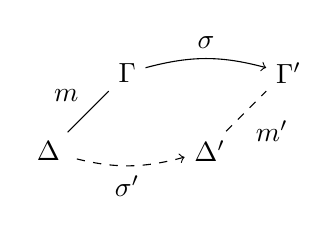
\begin{tikzpicture}
    \node (Γ) at (1,1) {$\Gamma$};
    \node (Γ') at (3,1) {$\Gamma\mathrlap'$};
    \node (Δ) at (0,0) {$\Delta$};
    \node (Δ') at (2,0) {$\Delta\mathrlap'$};
    \path (Γ) edge[->,bend left=15] node[above] {$\sigma$} (Γ')
    edge[-] node[auto=right] {$m$} (Δ)
    (Δ') edge[-,dashed] node[auto=right] {$m'$} (Γ')
    edge[<-,dashed,bend left=15] node[below] {$\sigma'$} (Δ);
  \end{tikzpicture}
  \caption{Intuition for the contexts involved in the $\textit{rewind}$ operation.
    We identify an OPE $\Gamma \subseteq \Gamma'$,
    or substitution $\operatorname{Sub} \Gamma \; \Gamma'$,
    as a map $\sigma$ on terms from the context $\Gamma$ to $\Gamma'$.
    Then, given a modal accessibility relation $m : \Delta \lhd \Gamma$,
    $\Delta$ being some past world,
    $\textit{rewind} \; m \; \sigma$ yields $\sigma'$ and $m'$
    for some context $\Delta'$.
    \label{fig:rewind}}
\end{figure}

For substitutions - and later environments - we note that both
can be seen as replacement lists of items for each type in a context.
Thus we choose to define them as concrete instances of a type $\Rpl$,
parametric over some function
$F : \textit{Type} \to \textit{Context} \to \textbf{Set}$
and defined inductively as
\begin{equation*}
  \inferrule{ }{\cdot : \Rpl \cdot \; \Delta} \quad
  \inferrule{\sigma : \Rpl \Gamma \; \Delta \\ x : F \; A \; \Delta}
            {\sigma, x : \Rpl \; (\Gamma, A) \; \Delta} \quad
  \inferrule{\sigma : \Rpl \Gamma \; \Delta \\ m : \Delta\lhd\Delta'}
            {\operatorname{lock} \sigma \; m : \Rpl \; (\Gamma, \lock) \; \Delta'}
\end{equation*}
This helps unify some of the calculus parameters,
and avoids having some parameters depend on
e.g. the definition of terms which in turn depends on other parameters.
Substitutions may then be defined as
$\operatorname{Sub} \coloneqq \operatorname{Rpl}_F$
with $F \; A \; \Gamma \coloneqq \Gamma \vdash A$.

With the exception of the $\operatorname{lock}$ constructor
the definition of $\Rpl$ is as for substitutions in STLC.
Adding the alternate constructor
$\operatorname{lift}_\lock : \Rpl \Gamma \; \Delta \to \Rpl \; (\Gamma, \lock) \; (\Delta, \lock)$
to STLC substitutions would allow them to represent local substitutions
in any of the ``worlds'' delimited by locks in the context.
Instead, $\operatorname{lock}$ with an argument $m : \Delta\lhd\Delta'$
(as used in \cite{valliappan22})
makes it possible to unify substitutions and \emph{modal transformations},
where locks are removed and added from contexts as permitted by $(\lhd)$,
and which are needed to describe the effect of unboxing.

With this choice of $\operatorname{lock}$ we make use of the parameter
$$ \lhd_\lock : \forall\Gamma. \, \Gamma \lhd \Gamma, \lock $$
in order to be able to define the identity substitution
$\textit{id}_s : \forall\Gamma. \, \operatorname{Sub} \Gamma \; \Gamma$.

As for OPE:s we define
$\textit{subst} : \operatorname{Rpl} \Gamma \; \Delta \to \Gamma \vdash t : A \to \Delta \vdash t : A$,
using the parameter
$$ \textit{rewind} : (m : \Gamma'\lhd\Gamma) \to (\sigma : \operatorname{Rpl} \Gamma \; \Delta) \to \exists \Delta'. \, \Delta'\lhd\Delta \times \operatorname{Rpl} \Gamma' \; \Delta' $$

The equational theory of $\lambda_\text{PFM}$ is given in figure~\ref{fig:eq-theory},
where reflexivity, symmetry, transitivity and congruence rules,
which ensure that $(\sim)$ is an equivalence relation,
have been omitted.
The notation $t \sim s$ says that the terms $t$ and $s$
are equal up to the conversion.

\begin{figure}
  \centering
  \begin{align*}
    \llap{$\beta$ equivalence:}& \quad
    \inferrule{\Gamma, A \vdash t : B \\ \Gamma \vdash s : A}{(\lambda. \, t) \; s \sim t[s]} \quad
    \inferrule{\Delta, \lock \vdash t : A \\ m : \Delta \lhd \Gamma}{\unbox \; (\operatorname{box} t) \; m \sim \textit{subst} \; (\operatorname{lock} \textit{id}_s \; m) \; t} \\
    \llap{$\eta$ equivalence:}& \quad
    \inferrule{\Gamma \vdash t : A \to B}{t \sim \lambda. \, (\textit{wk} \; (\operatorname{weak} \textit{id}_\subseteq) \; t) \; (\operatorname{var} \operatorname{zero})} \quad
    \inferrule{\Gamma \vdash t : \Box A}{t \sim \operatorname{box} \; (\operatorname{unbox} t \; \lhd_\lock)}
  \end{align*}
  \caption{Equational theory of $\lambda_\text{PFM}$.
    The rules for lambda abstraction are as for STLC.
    In the $\lambda$-$\beta$-conversion rule,
    $t[s]$ denotes applying a singleton substitution to $t$:
    Replacing the zeroth variable with $s$
    and decrementing all other de Bruijn indices.
    \label{fig:eq-theory}}
\end{figure}

\section{Normalization algorithm}\label{sec:normalization}

We provide a NbE algorithm based on a possible worlds model.
Normal and neutral forms are defined mutually as:
\begin{gather*}
  \inferrule{x : \text{Ne} \; \Gamma \; \iota}{\operatorname{ne} x : \text{Nf} \; \Gamma \; \iota} \quad
  \inferrule{x : \text{Nf} \; (\Gamma, A) \; B}{\operatorname{abs} x : \text{Nf} \; \Gamma \; (A \to B)} \quad
  \inferrule{x : \text{Nf} \; (\Gamma, \lock) \; A}{\operatorname{box} x : \text{Nf} \; \Gamma \; (\Box A)} \\
  \inferrule{x : A \in \Gamma}{\operatorname{var} x : \text{Ne} \; \Gamma \; A} \quad
  \inferrule{x : \text{Ne} \; \Gamma \; (A \to B) \\\\ y : \text{Nf} \; \Gamma \; A}
            {x \; y : \text{Ne} \; \Gamma \; B} \quad
  \inferrule{x : \text{Ne} \; \Delta \; (\Box A) \\ m : \Delta\lhd\Gamma}{\operatorname{unbox} x \; m : \text{Ne} \; \Gamma \; A}
\end{gather*}
The normal forms are $\beta$-normal - no $\beta$-reductions are possible -
and $\eta$-long - all variables are maximally applied and unboxed,
as the $\operatorname{ne}$ constructor only permits neutral values of the base type.

As done in \cite{valliappan22}, we choose contexts for worlds,
weakenings for the intuitionistic accessibility relation between worlds, and
$(\lhd)$ for the modal accessibility relation.
(The intuitionistic accessibility relation should be thought of as
relating two worlds $w_1$ and $w_2$ if $w_2$ has as much or more knowledge than $w_1$;
for worlds as contexts this means all assumptions in $w_1$ should be present in $w_2$ too.)
Then we interpret types in the model as
\begin{equation}\label{eq:sem-values}
  \begin{split}
  \llbracket \iota \rrbracket_\Gamma &\coloneqq \text{Nf} \; \Gamma \; \iota \\
  \llbracket A \to B \rrbracket_\Gamma &\coloneqq \forall \Delta. \, \Gamma \subseteq \Delta \to \llbracket A \rrbracket_\Delta \to \llbracket B \rrbracket_\Delta \\
  \llbracket \Box A \rrbracket_\Gamma &\coloneqq \forall \Gamma', \Delta. \, \Gamma \subseteq \Gamma' \to \Gamma'\lhd\Delta \to \llbracket A \rrbracket_\Delta
  \end{split}
\end{equation}
and contexts as environments, i.e. lists of semantic values, using $\operatorname{Rpl}$,
$$ \llbracket \Gamma \rrbracket_\Delta \coloneqq \operatorname{Rpl}_{\llbracket-\rrbracket} \Gamma \; \Delta $$
We have monotonicity for semantic values and environments,
i.e. we have
$wk_A : \Delta \subseteq \Delta' \to \llbracket A \rrbracket_\Delta \to \llbracket A \rrbracket_\Delta'$ and
$wk_\Gamma : \Delta \subseteq \Delta' \to \llbracket \Gamma \rrbracket_\Delta \to \llbracket \Gamma \rrbracket_\Delta'$.

The definition of evaluation, reification and reflection is given in figure~\ref{fig:nbe}.
Variable lookup is as for STLC -
the \textsc{Var} rule does not permit access across lock delimiters in the context,
thus the $\operatorname{lookup}$ function just has to read
the variable value from its place in the local environment.
The normalization function may then be given as
\begin{definition}[Normalization by Evaluation]
  Given a term $\Gamma \vdash t : A$,
  normalization yields a normal form $\operatorname{Nf} \; \Gamma \; A$,
  $$ \textit{nf} \; t \coloneqq \, \downarrow^A (\llbracket t \rrbracket \; \textit{id}_e) $$
  where $\textit{id}_e$ is the identity environment.
\end{definition}
The algorithm can be summarized as follows:
Evaluation proceeds as for an interpreter,
except closures take an extra OPE argument -
this allows conjuring fresh variables under binders
when reifying functions.
Then the resulting semantic value is reified back to its normal form.
When reifying a box or function,
evaluation resumes with the boxed term,
or the closure applied to a neutral form corresponding to the argument type,
respectively.

\begin{figure}
  \centering
  \begin{align*}
    &\mathrlap{\text{Evaluation} \quad \llbracket-\rrbracket : \Gamma \vdash t : A \to \forall\Delta. \, \llbracket\Gamma\rrbracket_\Delta \to \llbracket A \rrbracket_\Delta} &&\\
    &\llbracket x \rrbracket \; \gamma &&\coloneqq \text{lookup } x \text{ in } \gamma \\
    &\llbracket \lambda. \, t \rrbracket \; \gamma &&\coloneqq \lambda w \; \hat a.\, \llbracket t \rrbracket \; (\operatorname{wk}_{\widehat\Gamma} w \; \gamma, \hat a) \\
    &\llbracket t \; s \rrbracket \; \gamma &&\coloneqq \llbracket t \rrbracket \; \textit{id}_\subseteq \; (\llbracket s \rrbracket \; \gamma) \\
    &\llbracket \operatorname{box} t \rrbracket \; \gamma &&\coloneqq \lambda w \; m.\, \llbracket t \rrbracket \; (\operatorname{lock} \; (\operatorname{wk}_{\widehat\Gamma} w \; \gamma) \; m) \\
    &\llbracket \operatorname{unbox} t \; m \rrbracket \; \gamma &&\coloneqq \llbracket t \rrbracket \; \widehat\Delta \; \textit{id}_\subseteq \; m' \quad \text{where } m' , \widehat\Delta = \textit{rewind} \; m \; \gamma \\
    &\mathrlap{\text{Reification} \quad \downarrow^A : \llbracket A \rrbracket_\Gamma \to \operatorname{Nf} \; \Gamma \; A} &&\\
    &\downarrow^\iota a &&\coloneqq a \\
    &\downarrow^{A \to B} a &&\coloneqq \operatorname{abs} \; (\downarrow^B (a \; (\operatorname{weak} \textit{id}_\subseteq) \; (\uparrow^A (\operatorname{var} \operatorname{zero})))) \\
    &\downarrow^{\Box A} a &&\coloneqq \operatorname{box} \; (\downarrow^A (a \; \textit{id}_\subseteq \; \lhd_\lock)) \\
    &\mathrlap{\text{Reflection} \quad \uparrow^A : \operatorname{Ne} \; \Gamma \; A \to \llbracket A \rrbracket_\Gamma} &&\\
    &\uparrow^\iota x &&\coloneqq \operatorname{nt} a \\
    &\uparrow^{A \to B} x &&\coloneqq \lambda w \; a.\, \uparrow^B ((\operatorname{wk}_{\operatorname{Ne}} w \; x) \; (\downarrow^A a)) \\
    &\uparrow^{\Box A} x &&\coloneqq \lambda a.\, \uparrow^B (\operatorname{unbox} \; (\operatorname{wk}_{\operatorname{Ne}} w \; x) \; m)
  \end{align*}
  \caption{Evaluation, reification and reflection definitions. \label{fig:nbe}}
\end{figure}

Here we have chosen the possible worlds inspired interpretation of $\Box A$,
instead of the syntax-directed approach of
$$ \llbracket \Box A \rrbracket_\Gamma = \llbracket A \rrbracket_{\Gamma, \lock}$$
one reason being that the $\unbox$ case of evaluation then would require
being able to apply the equivalent of a $\operatorname{lock} \textit{id} \; m$ substitution
on semantic values, in addition to weakening,
whereas currently no such thing is needed,
as the $m$ instead goes directly in $\unbox$ when reflecting.

\section{Correctness}\label{sec:correctness}

We define the composition of two $\operatorname{Rpl}$:s, which,
while not appearing in the normalization algorithm,
is used in the proof of its correctness.
\begin{definition}[Composition of $\operatorname{Rpl}$:s]\label{def:composition}
  For $\sigma : \operatorname{Rpl}_F \Gamma \; \Delta$
  and $\delta : \operatorname{Rpl}_G \Delta \; \Xi$,
  $F$ not necessarily equaling $G$,
  their composition $\sigma \circ \delta : \operatorname{Rpl}_G \Gamma \; \Xi$
  is given by
  \begin{align*}
    \cdot \circ \delta &\coloneqq \cdot \\
    (\sigma , a) \circ \delta &\coloneqq (\sigma \circ \delta) , \textit{apply} \; \delta \; a \\
    \operatorname{lock} \sigma \; m \circ \delta &\coloneqq \operatorname{lock} \; (\sigma \circ \delta') \; m'
    \quad \text{where } m' , \delta' = \textit{rewind} \; m \; \delta
  \end{align*}
  where the definition is generic over a function
  $\textit{apply} : \forall A \; \Gamma \; \Delta.\, \operatorname{Rpl}_G \Gamma \; \Delta \to F \; A \; \Gamma \to G \; A \; \Delta$.
  E.g. for substitution/substitution composition
  $\textit{apply}$ will be $\textit{subst}$.
\end{definition}
As the source context $\Gamma$ of $\sigma \circ \delta$ is the same as for $\sigma$,
composition will preserve the inductive shape of $\sigma$,
but differ i.a. in the $(-,-)$ constructor contents
where $\delta$ is $\textit{apply}$:ed.

Soundness and completeness of the conversion relation
has been proved with respect to possible worlds,
with the addition of the following calculus parameters
\begin{itemize}
\item Rewinding $\operatorname{lock} \sigma \; m$
  with a modal accessibility relation $\Gamma \lhd \Gamma, \lock$
  should work as expected, i.e. give back $m$ and $\sigma$:
  $$ \textit{rewind-$\lhd_\lock$} : \forall m, \sigma. \, \textit{rewind} \lhd_\lock (\operatorname{lock} \sigma \; m) \equiv m , \sigma $$
  and the same for $\textit{rewind}_\subseteq$ on $\operatorname{lift}_\lock$.
\item The operation $\textit{rewind}$ distributes over composition:
  \begin{align*}
    \textit{rewindPres-$\circ$} &: (m : \Delta\lhd\Gamma) \to (\sigma_1 : \operatorname{Rpl} \Gamma \; \Gamma') \to (\sigma_2 : \operatorname{Rpl} \Gamma' \; \Gamma'') \\
    &\to
    \begin{array}[t]{@{}l@{}l@{}}
      \text{let } & m' , \sigma_1' = \textit{rewind} \; m \; \sigma_1 \\
      & m'' , \sigma_2' = \textit{rewind} \; m' \; \sigma_2 \\
      \text{in } & \textit{rewind} \; m \; (\sigma_1 \circ \sigma_2) \equiv m'' , \sigma_1' \circ \sigma_2'
    \end{array}
  \end{align*}
  and likewise for $\textit{rewind}_\subseteq$.
\item $\textit{rewind}$ should preserve identity:
  $$ \textit{rewindPresId} : (m : \Delta\lhd\Gamma) \to \textit{rewind} \; m \; \textit{id} \equiv m , \textit{id} $$
  and likewise for $\textit{rewind}_\subseteq$.
\item $\textit{rewind}$ should commute with weakening and substitution composition:
  \begin{align*}
    &\textit{rewindWk} &&: (m : \Delta\lhd\Gamma) \to (\sigma : \operatorname{Rpl} \Gamma \; \Gamma') \to (w : \Gamma' \subseteq \Gamma'') \\
    &&&\to
    \begin{array}[t]{@{}l@{}l@{}}
      \text{let } & m' , \sigma' = \textit{rewind} \; m \; \sigma \\
      & m'' , w' = \textit{rewind}_\subseteq \; m' \; w \\
      \text{in } & \textit{rewind} \; m \; (\textit{wk} \; w \; \sigma) \equiv m'' , \textit{wk} \; w' \; \sigma'
    \end{array} \\
    &\textit{rewindTrim} &&: (m : \Delta\lhd\Gamma) \to (w : \Gamma \subseteq \Gamma') \to (\sigma : \operatorname{Rpl} \Gamma' \; \Gamma'') \\
    &&&\to
    \begin{array}[t]{@{}l@{}l@{}}
      \text{let } & m' , w' = \textit{rewind}_\subseteq \; m \; w \\
      & m'' , \sigma' = \textit{rewind} \; m' \; \sigma \\
      \text{in } & \textit{rewind} \; m \; (\textit{trim} \; w \; \sigma) \equiv m'' , \textit{trim} \; w' \; \sigma'
    \end{array}
  \end{align*}
  where $\textit{wk} : \Delta\subseteq\Delta' \to \operatorname{Sub} \Gamma \; \Delta \to \operatorname{Sub} \Gamma \; \Delta'$ and
  $\textit{trim} : \Gamma\subseteq\Gamma' \to \operatorname{Sub} \Gamma \; \Delta \to \operatorname{Sub} \Gamma' \; \Delta$
  is substitution and weakening composition and vice versa, respectively.
\end{itemize}
These enable proving of the necessary weakening and substitution laws.
Indeed, most show up in the goals when proving the $\unbox$ cases of the laws.

\subsection{Completeness}

Completeness states that a term is convertible to its normal form.
\begin{theorem}[Completeness]
  If $\Gamma \vdash t : A$, then $t \sim \ulcorner \textit{nf} \; t \urcorner$.
\end{theorem}

The proof is an extension of the corresponding proof for STLC \cite{kovacs17},
and established by a \emph{Kripke logical relation} \cite{plotkin73}
between terms and semantic values:
\begin{align*}
  (\simeq^A) &\subseteq \Gamma \vdash A \times \llbracket A \rrbracket_\Gamma \\
  t \simeq^\iota \hat t &\coloneqq t \sim \ulcorner \hat t \urcorner \\
  t \simeq^{A \to B} \hat t &\coloneqq (w : \Gamma \subseteq \Delta) \to \forall a : \Delta \vdash A, \hat a : \llbracket A \rrbracket_\Delta.\, a \simeq \hat a \\
  &\qquad \to \operatorname{app} \; (\textit{wk} \; w \; t) \; a \simeq \hat t \; w \; \hat a \\
  t \simeq^{\Box A} \hat t &\coloneqq (w : \Gamma \subseteq \Gamma') \to (m : \Gamma' \lhd \Delta)
  \to \operatorname{unbox} \; (\textit{wk} \; w \; t) \; m \simeq \hat t \; w \; m
\end{align*}
It is \emph{logical} in the sense that terms and semantic values of box/function types
are related iff the results from unboxing/applying both to related terms and values, are related;
``Kripke'' means that we may first extend the context with a weakening.
Notice how the definition of the logical relation has the same shape
as that of semantic values, see equation \eqref{eq:sem-values}.
We will prove for each inductive step of normalization that $(\simeq)$ is maintained;
just as $\textit{nf}$ always returns a normal form through reification,
after reification we will get a $(\sim)$ out of $(\simeq)$.

We extend $(\simeq)$ to a relation $(\simeq_\text{ctx})$
between substitutions and environments elementwise related by $(\simeq)$,
and show that
the interpretations of a term in related substitutions and environments are related,
the so called \emph{fundamental theorem} of the logical relation:
\begin{lemma}[Fundamental theorem]
  If $t : \Gamma \vdash A$, $\sigma : \operatorname{Sub} \; \Gamma \; \Delta$,
  $\delta : \operatorname{Env} \; \Gamma \; \Delta$
  and $\sigma \simeq_\text{ctx} \delta$,
  then $\textit{subst} \; \sigma \; t \simeq \llbracket t \rrbracket \; \delta$.
\end{lemma}
\begin{proof}
  By induction on $t$.
  For the case of $t = \operatorname{box} \; s$, it needs to be shown that for all
  $w : \Delta \subseteq \Delta'$, $m : \Delta' \lhd \Xi$,
  \begin{equation*}
    \operatorname{unbox} \; (\operatorname{box} \; (\textit{wk} \; (\operatorname{lift}_\lock \; w) \; (\textit{subst} \; (\operatorname{lock} \; \sigma \; \lhd_\lock) \; s)))
    \simeq \llbracket s \rrbracket \; (\operatorname{lock} \; (\textit{wk} \; w \; \delta) \; m)
  \end{equation*}
  The induction hypothesis gives
  $$ \textit{subst} \; (\operatorname{lock} \; (\textit{wk} \; w \; \sigma) \; m) \; s \simeq \llbracket s \rrbracket \; (\operatorname{lock} \; (\textit{wk} \; w \; \delta) \; m) $$
  which we compose with a conversion proof on the left
  \begin{equation*}
    \begin{split}
      &\Box\text{-}\beta \; (\textit{wk} \; (\operatorname{lift}_\lock \; w) \; (\textit{subst} \; (\operatorname{lock} \; \sigma \; \lhd_\lock) \; s)) \; m \\
      &\quad : \operatorname{unbox} \; (\operatorname{box} \; (\textit{wk} \; (\operatorname{lift}_\lock \; w) \; (\textit{subst} \; (\operatorname{lock} \; \sigma \; \lhd_\lock) \; s))) \\
      &\qquad \sim \textit{subst} \; (\operatorname{lock} \; \textit{id} \; m) \; (\textit{wk} \; (\operatorname{lift}_\lock \; w) \; (\textit{subst} \; (\operatorname{lock} \; \sigma \; \lhd_\lock) \; s))
    \end{split}
  \end{equation*}
  Here the term on the right side of $(\sim)$ does not immediately match up
  with the left side of $(\simeq)$ in the IH,
  however one can show that they are in fact equal
  using $\textit{rewind-/rewind$_\subseteq$-}\lhd_\lock$ and substitution laws.

  For the $t = \operatorname{unbox} \; s \; m$ case,
  it suffices to rewind the proof of $\sigma\simeq_\text{ctx}\delta$ by $m$ to get
  $$ \textit{rewind} \; m \; \sigma \simeq_\text{ctx} \textit{rewind} \; m \; \delta $$
  and apply the IH on it and $s$.
\end{proof}

Similarly, we show that reification and reflection also respect $(\simeq)$.
\begin{lemma}
  Reification and reflection respect $(\simeq)$:
  \begin{enumerate}
    \renewcommand{\theenumi}{\alph{enumi}}
  \item If $t : \Gamma \vdash A$, $\hat t : \llbracket A \rrbracket_\Gamma$
    and $t \simeq \hat t$ then $t \sim \ulcorner \downarrow\hat t \urcorner$.
  \item If $t : \operatorname{Ne} \Gamma \; A$ then $\ulcorner t \urcorner \simeq \, \uparrow t$.
  \end{enumerate}
\end{lemma}
\begin{proof}
  By induction on $A$.
  (We only show the $\Box A$ case of (a),
  with the rest left as an exercise to the reader.)
  The proof of $t \simeq \hat t$ says unboxing of $t$ and $\hat t$ respects $(\simeq)$.
  Choosing $w = \textit{id}_\subseteq$ and $m = \lhd_\lock$
  and applying the IH on the result yields
  $$ \operatorname{unbox} \; (\textit{wk} \; \textit{id}_\subseteq \; t) \; \lhd_\lock \simeq \ulcorner \downarrow (\hat t \; \textit{id}_\subseteq \; \lhd_\lock) \urcorner $$
  where $\textit{wk} \; \textit{id}_\subseteq \; t = t$.
  Combining this with the $\Box\text{-}\eta$ conversion rule for $t$, i.e.
  $$ t \sim \operatorname{box} \; (\operatorname{unbox} \; t \; \lhd_\lock) $$
  using transitivity and congruence under $\operatorname{box}$
  of the conversion relation gives the goal.
\end{proof}

The fundamental theorem,
using $\textit{id}_s$ and $\textit{id}_e$ for substitution and environment,
may then be combined with the reification lemma
to conclude the completeness proof.

One detail remains, however.
Depending on how $(\simeq_\text{ctx})$ is defined we may not be able to rewind it.
We know only how to rewind OPE:s and $\operatorname{Rpl}$:s,
not arbitrary data types, without taking more rewind functions as parameters.
Thus we let $(\simeq_\text{ctx}) \coloneqq \operatorname{Rpl}_{A\simeq\widehat A}$ where
$$ A\!\simeq\!\widehat A \; A \; \Gamma \coloneqq \exists t : \Gamma \vdash A, \hat t : \llbracket A \rrbracket_\Gamma.\, t \simeq \hat t $$
is triplet of a term, a semantic value, and a proof that the two are related.
The substitution may be recouped by mapping the $\operatorname{Rpl}$
with a function that picks the $t$ out of each $A\!\simeq\!\widehat A$,
likewise for the environment.
For the proof of the $\operatorname{unbox}$ case of the fundamental theorem,
we need an additional calculus parameters
\begin{itemize}
\item Rewind should commute with $\textit{map}_{\operatorname{Rpl}}$:
  \begin{multline*}
  \textit{rewindCommMap} : \forall (f : \forall A, \Gamma.\, F \; A \; \Gamma \to G \; A \; \Gamma), m, \sigma : \operatorname{Rpl}_F \; \Gamma \; \Delta. \\
  \pi_1 \; (\textit{rewind} \; m \; \sigma) \equiv \pi_1 \; (\textit{rewind} \; m \; (\textit{map} \; f \; \sigma)) \\
  \land \textit{map} \; f \; (\pi_2 \; (\textit{rewind} \; m \; \sigma)) \equiv \pi_2 \; (\textit{rewind} \; m \; (\textit{map} \; f \; \sigma))
  \end{multline*}
  where $\pi_1$ and $\pi_2$ is the first and second projections of the product type.
\end{itemize}
The parameter $\textit{rewindCommMap}$ enables us
to get the rewound substitution/environment
from a rewound proof of $\sigma \simeq_\text{ctx} \delta$.
It should be noted that we expect the equivalence to hold a priori,
since a $\textit{rewind}$ instantiation cannot observe
the contents of the parametric $\operatorname{Rpl}$,
as explained in \citetitle{wadler89} \cite{wadler89}.
We still need to take them as parameters however,
in order to convince Agda.

\subsection{Soundness}

For two convertible terms,
soundness expresses that normalization maps them to the same normal form.
\begin{theorem}[Soundness]
  If $\Gamma : t \sim t'$, then $\textit{nf} \; t = \textit{nf} \; t'$.
\end{theorem}

The standard technique for proving soundness of STLC \cite{altenkirch95,kovacs17}
uses a so called \emph{presheaf model},
where terms are interpreted as \emph{natural transformations}
between semantic contexts and semantic types.
Concretely, what needs to be changed in order to ensure
our possible worlds model is also a presheaf model,
is to add \emph{naturality} conditions to the interpretation of types.
Recall the interpretation of box types from equation \eqref{eq:sem-values}:
$$ \llbracket \Box A \rrbracket_\Gamma \coloneqq \forall \Gamma', \Delta. \, \Gamma \subseteq \Gamma' \to \Gamma'\lhd\Delta \to \llbracket A \rrbracket_\Delta $$
We constrain each box value $\hat a : \llbracket \Box A \rrbracket_\Gamma$
(and similarly for function values,)
to fulfill for all $w : \Gamma \subseteq \Gamma'$, $m : \Gamma' \lhd \Delta$ and $w' : \Delta \subseteq \Delta'$,
$$ \hat a \; (w \circ w'') \; m' = \textit{wk}_{\widehat A} \; w' \; (\hat a \; w \; m) \quad \text{where } m' , w'' = \textit{rewind}_\subseteq \; m \; w' $$
i.e. semantic boxes should commute with weakenings.
This allows us to prove naturality for evaluation, reification and reflection.

For proving soundness, since normalization is evaluation followed by reification,
it suffices to show the following lemma:
\begin{lemma}[Evaluation is sound w.r.t. conversion]
  Given two terms $\Gamma \vdash t \; t' : A$ such that $t \sim t'$
  and an environment $\gamma : \operatorname{Env} \; \Gamma \; \Delta$,
  we have
  $$ \llbracket t \rrbracket \; \gamma = \llbracket t' \rrbracket \; \gamma $$
\end{lemma}
The proof is by induction on $t \sim t'$.
The $\Box\text{-}\eta$ equivalence case -
where $t'$ is $\operatorname{box} \; (\operatorname{unbox} \; t \; \lhd_\lock)$ -
follows from naturality of evaluation and $\textit{rewind-}\lhd_\lock$.
(Though, since box types are interpreted as functions
of a weakening and modal accessibility relation,
we must first postulate function extensionality
in order to only have to show pointwise equality.)

For $\Box\text{-}\beta$ equivalence it needs to be shown that
$$ \llbracket t \rrbracket \; (\operatorname{lock} \; (\textit{wk}_{\widehat\Gamma} \; \textit{id}_\subseteq \; \gamma') \; m') = \llbracket \textit{subst} \; (\operatorname{lock} \; \textit{id}_s \; m) \; t \rrbracket \; \gamma $$
where $m' , \gamma' = \textit{rewind} \; m \; \gamma$.
We accomplish this using the fact that evaluating a substituted term
is the same as evaluating the raw term in a modified environment,
as summarized in the following lemma:
\begin{lemma}[Action of evaluation on substituted terms]
  If $\Gamma \vdash t : A$, $\sigma : \operatorname{Sub} \; \Gamma \; \Delta$
  and $\gamma : \operatorname{Env} \; \Delta \; \Xi$, then
  $$ \llbracket \textit{subst} \; \sigma \; t \rrbracket \; \gamma = \llbracket t \rrbracket \; (\sigma \circ \gamma) $$
\end{lemma}
Here the fact that composition between $\operatorname{Rpl}$:s of different types is defined,
see definition~\ref{def:composition}, comes into play,
where we let $\textit{apply} \coloneqq \lambda \gamma \; t.\, \llbracket t \rrbracket \; \gamma$ be evaluation
in order to compose substitutions and environments.
After applying the lemma it remains to show
$$ \llbracket t \rrbracket \; (\operatorname{lock} \; (\textit{wk}_{\widehat\Gamma} \; \textit{id}_\subseteq \; \gamma') \; m') = \llbracket t \rrbracket \; (\operatorname{lock} \; (\textit{id}_s \circ \gamma') \; m') $$
which follows from
$wk_e \; \textit{id}_\subseteq \; \gamma = \gamma = \textit{id}_s \circ \gamma$.

\section{Concrete Instantiations}\label{sec:instantiations}

In this section we give instantiations of $\lambda_\text{PFM}$
for the two concrete modal lambda calculi highlighted in \cite{valliappan22}.

\subsection{Intuitionistic K}

To obtain $\lambda_\text{IK}$ we let the modal accessibility relation be
as in \autoref{fig:m-ik},
i.e. $\Gamma$ extends $\Delta, \lock$ to the right without adding locks.

\begin{figure}
  \centering
  \begin{equation*}
    \inferrule{}{\operatorname{base} : \Gamma \lhd_{\lambda_\text{IK}} \Gamma, \lock} \qquad
    \inferrule{m : \Delta \lhd_{\lambda_\text{IK}} \Gamma}{\operatorname{snoc} m : \Delta \lhd_{\lambda_\text{IK}} \Gamma, A}
  \end{equation*}
  \caption{Modal accessibility relation for $\lambda_\text{IK}$. \label{fig:m-ik}}
\end{figure}

The implementation of $\textit{rewind}$ is straightforward:
\begin{equation*}
  \begin{split}
    \textit{rewind} \; \operatorname{base} \; (\operatorname{lock} \sigma \; m') &\coloneqq m' , \sigma \\
    \textit{rewind} \; (\operatorname{snoc} \; m) \; (\sigma , \_) &\coloneqq \textit{rewind} \; m \; \sigma
  \end{split}
\end{equation*}
All the remaining parameters are also simple -
with the exception of $\textit{rewindPresId}$ where we need an additional lemma:
\begin{lemma}
  If $\sigma : \operatorname{Rpl} \Gamma \; \Gamma'$ such that
  $\textit{wk} \; \textit{id}_\subseteq \; \sigma$,
  then for all $m : \Delta \lhd_\text{IK} \Gamma$
  $$ \textit{rewind} \; m \; (\textit{drop} \; \sigma) = \textit{rewind} \; m \; s $$
  where $\textit{drop} \coloneqq \textit{wk} \; (\operatorname{weak} \; \textit{id}_\subseteq)$.
\end{lemma}
What makes the lemma provable is that all IK modal accessibility relations,
($\lhd_\text{IK}$), start with a \lock (see the $\operatorname{base}$ constructor).
The function $\textit{drop}$ only affects
the part of the context to the left of the lock,
which will be removed by the $\textit{rewind}$ operation.

\section{Future Work}

One point to investigate is whether to replace OPE:s with renamings,
i.e. substitutions where the replacement terms are variables.
Not only would this remove
some $\textit{rewind}_\subseteq$/$\textit{rewind}$ repetition,
but it would also be a step toward being able to add the \emph{R axiom}
($A \to \Box A$).
\textcite{valliappan-r} showed that the condition
$$ R_m \subseteq R_i $$
on $R_i$ and $R_m$,
the intuitionistic and modal accessibility relation, respectively,
is sufficient for ensuring axiom R is satisfied in the model
(with the IR \textsc{Var} rule and corresponding OPE definition).
Unlike with OPE:s as given here,
the condition holds when picking renamings for $R_i$,
since renamings encapsulate lock weakenings.

\section{Conclusion}\label{sec:conclusion}

\printbibliography

\end{document}
